\chapter{Introduction}

\section{Background}

Machine learning will be used to analyse student accommodation bookings with a focus on the ability to reliably estimate revenue in order to determine when a contract will not be fulfilled. This will be completed utilising data from the property management system. \cite{Jain2006IntellectualPerspective}

\vspace{5mm}

A contract made in advanced between the student (customer) and the company defines the services that will be sold (the room) as well as the start and end date of the tenancy and the fix price the service will be sold at. In the case of student accommodation this contract is usually made a few months in advanced, in some cases before the student has finalized there plan to attend a specific university. Because of this the student withholds the right to cancel the contract before it is paid. The inherit uncertainty of the contract means there is no way for the company to definitively measure what the occupancy and sales of a given property will be in advanced since, they have to take on the risk of cancellation. This problem is not specific to the student accommodation industry, this is a problem of revenue management first identified by the aviation industry in 1966  (\cite{Chiang2007AnResearch})

\vspace{5mm}


Having the ability to predict with some degree of certainty whether or not a booking is going to be cancelled would allow for more accurate decisions about revenue management to be made and overcome some of the risk created with contract based booking system. Doing this using machine learning means that overtime the accuracy of the predictions can increase with better understanding of the data, new iterations of modelling and evaluation of the actual outcome when compared with the predicted outcome. The ability for machine learning algorithm to make accurate predictions on a given outcome depends on the data available to it the amount of the data and the accuracy and usability of the data in, the case of booking management a lot of data is stored about each booking made. Meaning that it should be possible with the correct classification techniques to make accurate predictions on the outcome of the booking



\section{Problem Statement}

In total for the year 2020 to 2021, 25 percent of all 14363 bookings made where cancelled, this accounts for over 20 million pounds in revenue loss from customers who completed the booking process and then cancelled before the contract was payed. There are a number of different reasons that account for each booking being cancelled that range from impact caused due to COVID and students not receiving there target grades. In most of these cases the student will then chose to stay at different accommodation resulting in the sale being lost. Producing a model that is able to predict which of these bookings will be cancelled in real time would then allow the business to take actions to try and prevent the student from cancelling there booking. Being able to prevent just 10 percent of users from cancelling would therefore create a potential gain of 2 million in revenue per year.  

\vspace{5mm}

On a small scale, recognising the characteristics that are common among cancelled bookings would be relatively simple; for example, looking at the percentage of cancelled bookings in the previous year, an approximate estimate of the number of bookings that would be cancelled this year could be estimated. Then, to figure out why these bookings were cancelled, look at what these bookings have in common. In this case, however, no amount of human analysis could possibly account for all of the factors, given that the organisation operates over 70,000 beds around the world. The fact that a student has the right to cancel a reservation up until a certain time period for a specified penalty means that it is the provider's duty to account for the inherent ambiguity of the contract . The most common method to solve this problem is to simply take the number number of bookings cancelled in the previous year and use that number as an average to measure the number of bookings expected to be cancelled in the current year. The problem with this approach is that it only considers one of the many factors (previous year figures), while the company actually keeps hundreds of data points for each booking. As a result, I'm attempting to use machine learning to solve this problem. Since the dataset I'm using comes directly from the company in question and includes actual data about students, I've removed all personal information. Instead, I'll refer to students and assets solely by their IDs, ensuring that both the company and the students remain anonymous.
    
\section{Aims and objectives}

By combining all relevant data points from previous years' bookings, I hope to create a model that can classify a booking into two distinct states: cancelled or not cancelled. It's important to not only build a model that predicts which bookings will be cancelled, but also to understand why bookings are cancelled by using the model to determine which features in the dataset have the greatest impact on whether or not a customer will cancel. This is critical in assisting the company in making business decisions based on the data in order to not only avoid the cancellation but also to understand what actions can be taken to reduce the number of cancellations in the future.

\vspace{5mm}

The first step in solving any machine learning problem is obtaining accurate and clean data; in most cases (including this one), this is the most difficult problem to solve because data is rarely stored in a way that makes it easy to read and analyse; in fact, data is frequently stored and then never used. As a result, I'm approaching the problem by first creating a data warehouse to store and analyse the data before creating a classification model \cite{SessionsTHEALGORITHMS}. This data warehouse will exist in the Azure cloud on top of Docker Containers with the code written in python, with the aim being to create a stream to import new booking data into the data warehouse hourly ensuring that it is stored in a way that makes it easy to use for model training. The aim is to integrate the classification model into the booking management system by creating a daily list of which customers are most likely to cancel there bookings to the managers of there respective properties along with the recommended actions to be taken to prevent the cancellation. Storing the data of the actions taken and weather or not it was successful can then be used to improve future iterations of the model

\section{Solution approach}

To create a classification model on the booking dataset, I'll use the AutoML feature of Azure ML Studio. I use Auto ML because it automates the process of cross validations and feature engineering, which significantly speeds up the model development process. AutoML is able to take advantage of the cloud resources made available to me through my company by running multiple models at the same time and increasing the speed with which individual models are executed. Bookings will be classified into two distinct groups: cancelled or not cancelled. This is a binary classification because there are only two states in which a booking can be classified. There are two types of classification approaches: supervised and unsupervised learning. This is an example of supervised learning because the expected values are known. Given a sample of data and desired outputs, the goal of supervised learning is to find a function that best approximates the relationship between input and output observed in the data.

 \begin{figure}[H]
 %\centering
 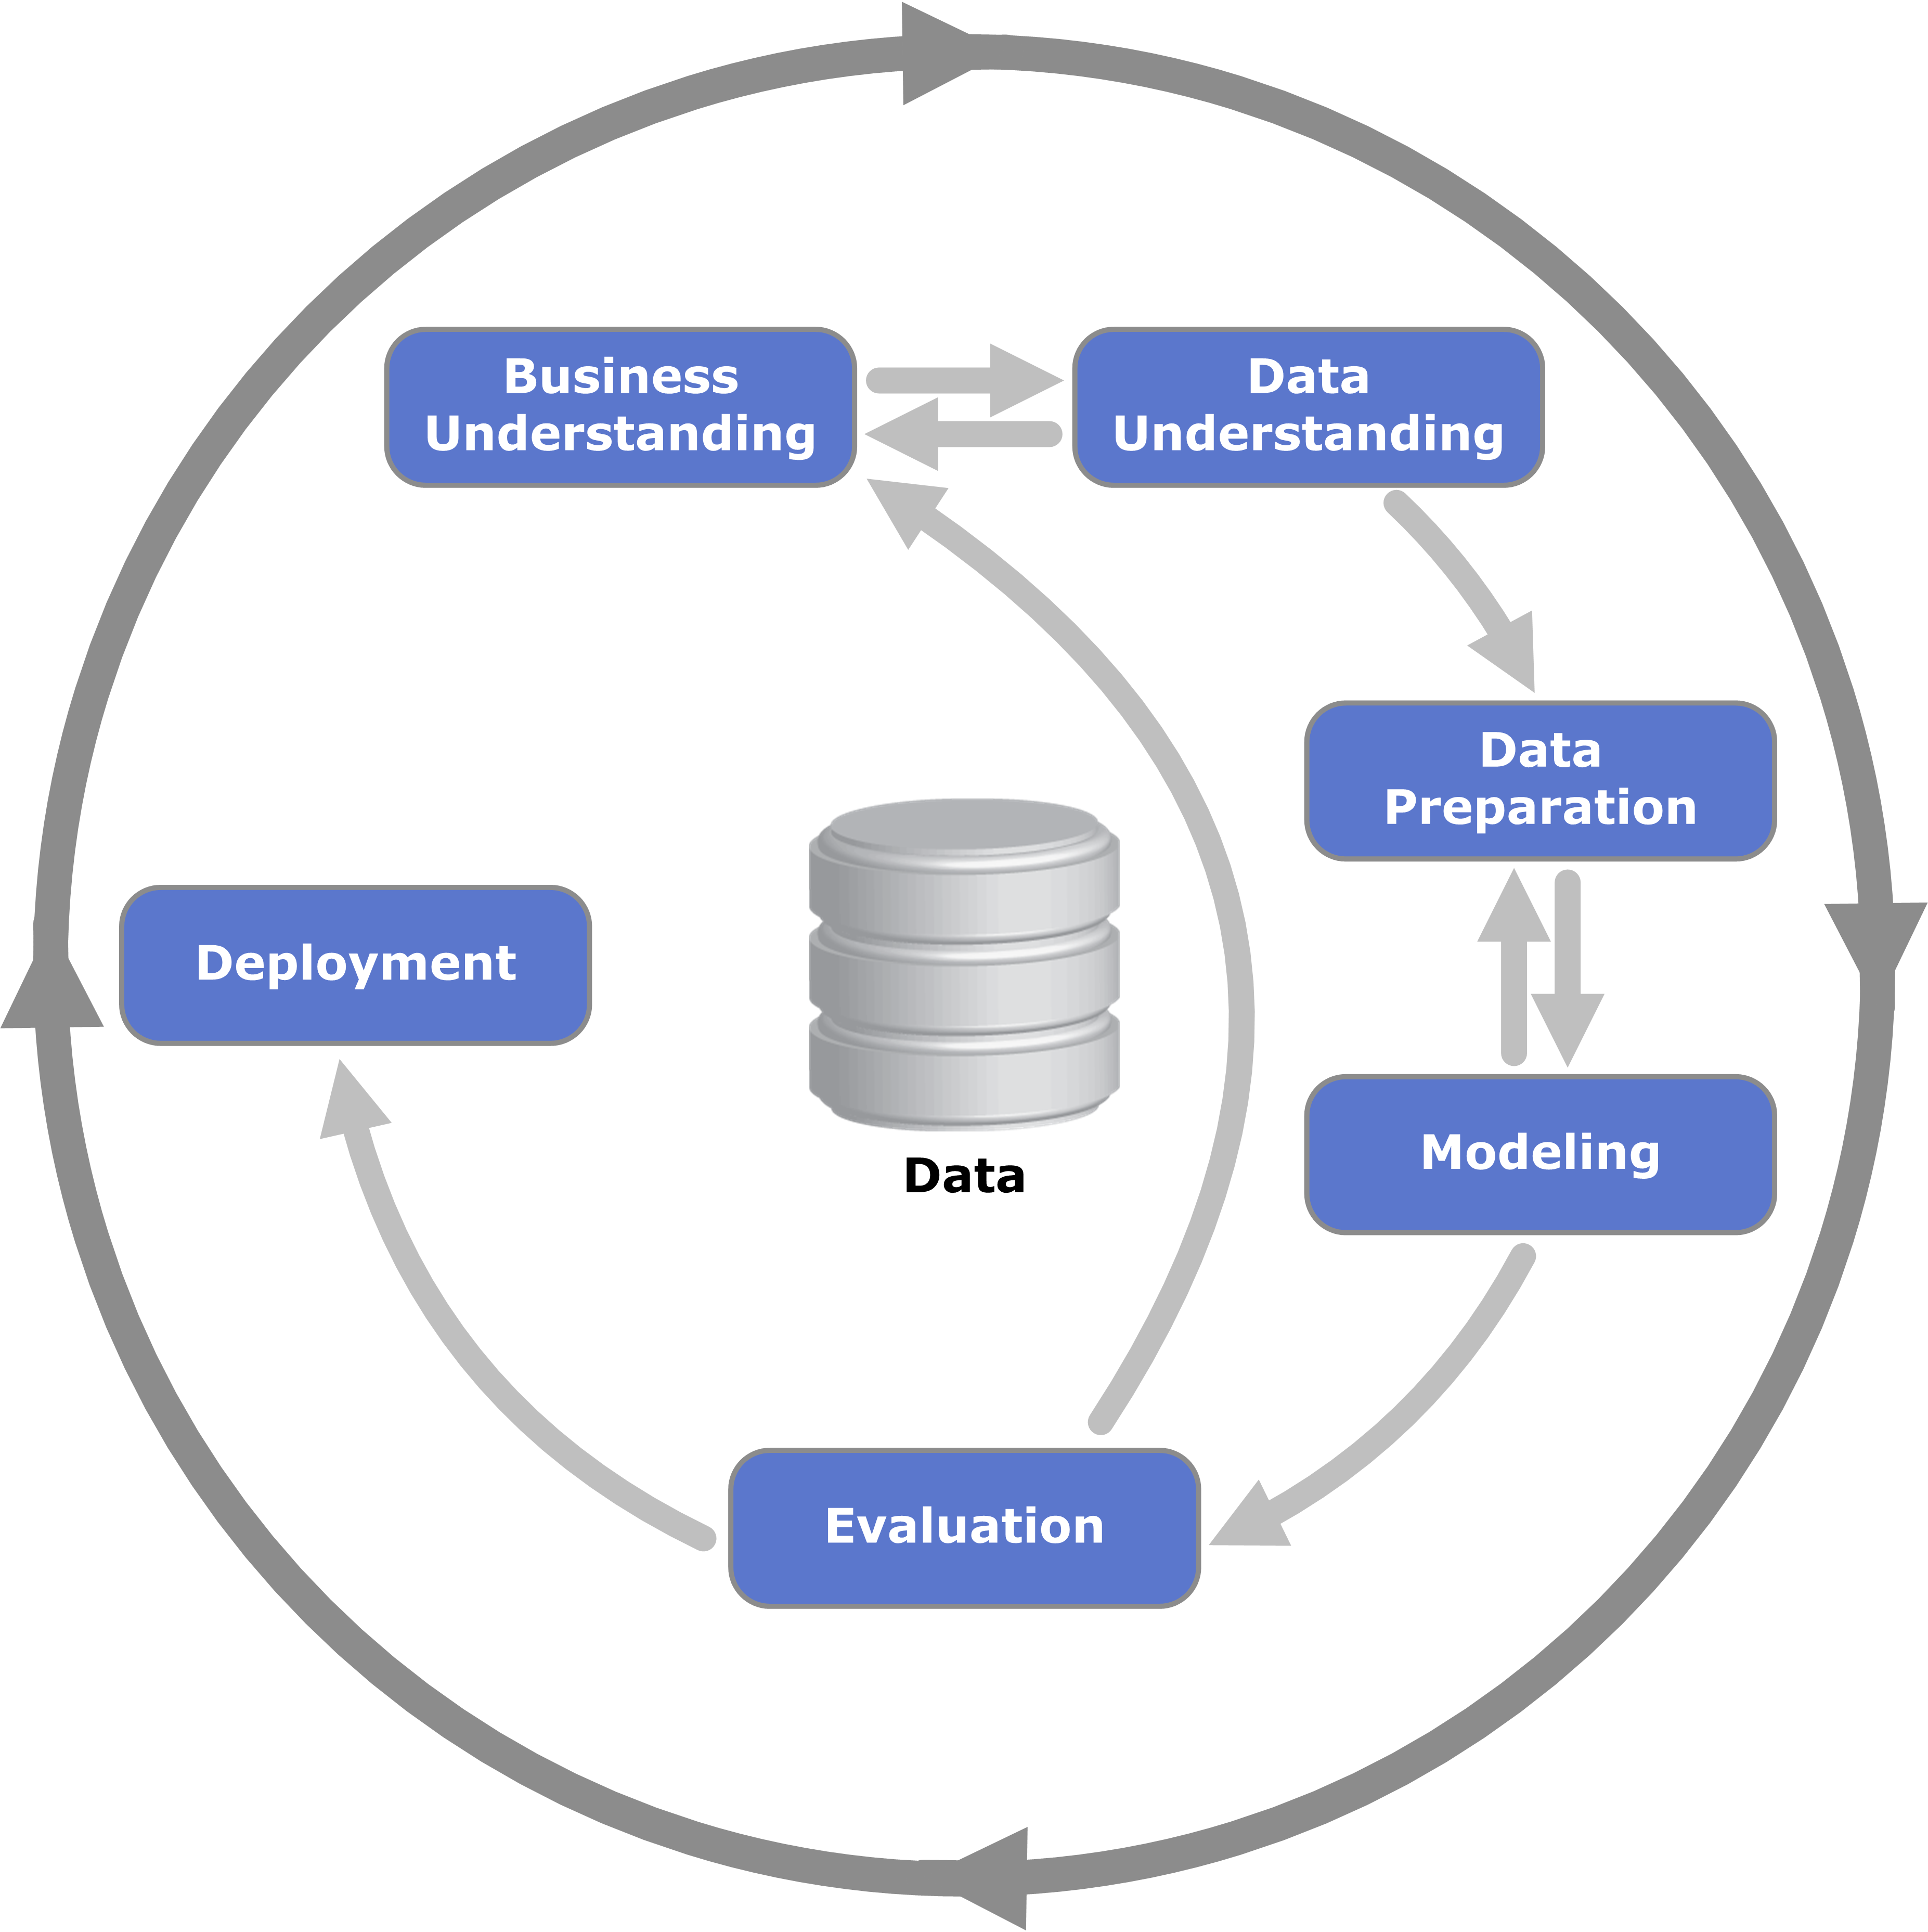
\includegraphics[width=10cm]{figures/CRISPDM_Process_Diagram.png}
 \caption{}
\end{figure} 


CRISP-DM is the most widely used data-mining model, according to current research, due to its numerous advantages, which solved existing data-mining problems \cite{Wirth2000CRISP-DMMining}. It works by breaking the problem down into six stages using the, as shown in figure 1.1: business understanding, data understanding, data preparation, modelling, evaluation, and deployment.

\vspace{5mm}

To determine the best approach to solving the problem, I began by consulting with company employees to gain a better understanding of the types of results that would be most effective, as well as the actions that can be taken to have the best chance of preventing a cancellation at the individual booking level. I discovered that it is critical that the results be presented in a way that employees can understand so that appropriate actions can be taken. Creating a table that ranked bookings by highest probability of cancellation was also discovered to be the best way to display the model's results. Another feature that I found to be important is the ability to retrain the model on new data and adjust the hyper tuning parameters, because the booking dataset is constantly being updated with new entries and it is constantly evolving.

\vspace{5mm}

One of the problems that needed to be solve was how to get access to data that is suitable for machine learning, this is the data preparation stage. This stage consistently requires the most time as seen in previous literature \cite{Zhang2003DataMining}. To perform machine learning, data needs to be accessible in a suitable format and stored appropriately. The current booking system behind the dataset in this research does not store the data in a way that is suitable for use in machine learning. Building a data warehouse allows for the data to be converted into an appropriate format for machine learning problems. An important aspect involves the ability of the data warehouse to update upon new bookings and allow instant access to the data, a feature of the data warehouse using azure cloud which was used in this project. The main technology used throughout the modeling process will be Azure ML studio as a framework to encapsulate all of the tools needed to complete a machine learning project, it allows for direct connection to the database for accessing the data through integrated Jupiter Notebooks. Use of Jupiter Notebooks in Python provides an environment for all of the data cleaning and preparation stages that need to be performed entirely within the azure cloud. The modeling stages are done in the same way by importing the AzureML Python SDK into the Jupiter Notebook. The Experiment class (azureml.core.experiment.Experiment) in the SDK is used to store and run the models within a logical resource group with the ability to add and remove different modeling iterations form the experiment as well as viewing the results, when a model is configured through AutoMLConfig (azureml.train.automl.automlconfig.AutoMLConfig) it is then added to the experiment and the run is executed in the cloud. Doing this process in the cloud helps to solve the the GDPR related problems of data access as the data is never stored on the local computer.

\begin{itemize}
\end{itemize}
\vspace{5mm}

The intended outcome of this research is to have the ability to rank bookings by the probability of them being cancelled, providing a platform to integrate the model results into the companies booking system. Doing this would allow the company to have the ability to input whether or not the prediction was correct. The model would then be able to be retrained based off the outcomes of the predictions, over time allowing for the models accuracy to be increased. 